\chapter{Architecture}

\setcounter{section}{4}
\setcounter{subsection}{0}

\label{sec:architecture}

When creating the architecture of a system that is supposed to provide a high grade of code re-usage is modularity and well defined abstraction layers important. By using the module pattern and letting each module have well defined responsibilities the system will be easier to maintain in the long run. The goal is to be able to move a module and put it in another project without any major modifications. This would allow a module to be replaced later on if the requirements of the system have changed. For this to work it is important that the module can function by itself. If it must interact with other modules this must be done through well defined interfaces. Another important aspect to keep in mind is that the whole system shall not crash just because one module fails. In order to fulfill these goals the design will be divided into components where each component can either be constructed by other components or have a primitive task itself. 

\subsection{System-level architecture}

The entire system can be divided into three separate components: a backend API, an API driver and the Javascript application itself. The backend API provides the Javascript application with data and the driver takes care of the abstraction in between. By utilizing a driver it becomes possible to replace the backend or frontend independently from each other. The user interacts with the Javascript application by either providing a URL to the system or in terms of user input such as clicking and pressing buttons. The application can at any time change the DOM (Document Object Model) to give the user feedback of the provided input actions. The DOM is the browser's representation of the elements on the page and is used when rendering it. An abstract view of the architecture seen from a system-level point of view can be seen in figure \ref{fig:system_design_abstract}.

Many other frameworks do not have the API driver as a bridge between the backend API and the Javascript application, making them tightly coupled together. For example, to change the backend from using AJAX requests to HTML5 websockets would in most cases require a redesign of the entire Javascript application. By letting the driver have a well defined interface the components can be replaced independent of each other. It also allows drivers to be re-used between project since the interface is the same independently on the application.

\begin{figure}[h!]
	\centerline{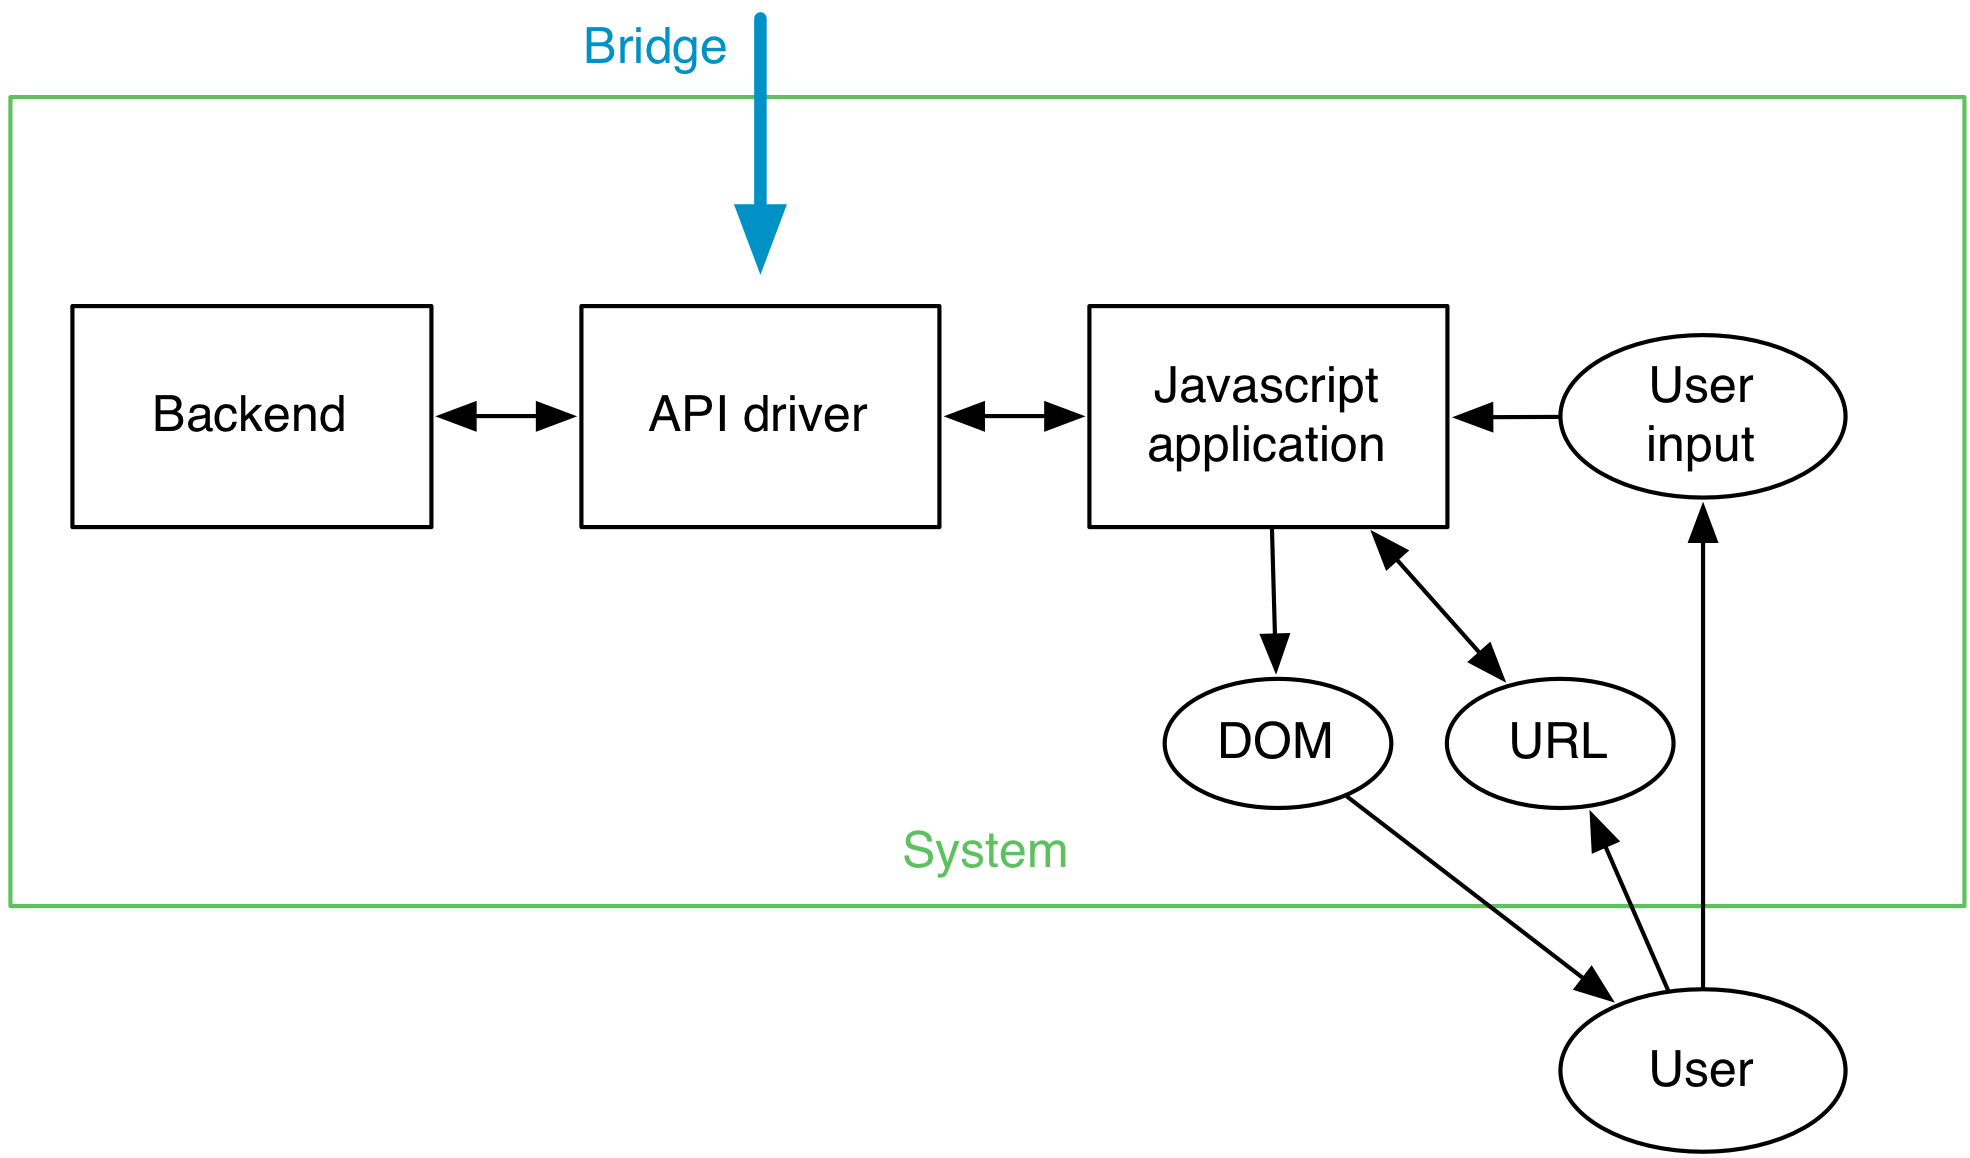
\includegraphics[width=100mm]{gfx/system_design_abstract.png}}
	\caption{The architecture seen from a system-level point of view.}
	\label{fig:system_design_abstract}
\end{figure}

\subsection{Application-level architecture}

The system architecture can be further refined. The Javascript application can itself be constructed by a number of other components including a router, a configuration as well as a number of modules and services. The router's task is to take the URL provided by the user and, depending on its value, load a specific module. This might imply that another module first has to be unloaded. The configuration provides an application-specific key-value-storage for global configuration properties. This is for example used to specify what API driver to use. The application-level architecture is described in figure \ref{fig:arch_app}.

\begin{figure}[h!]
	\centerline{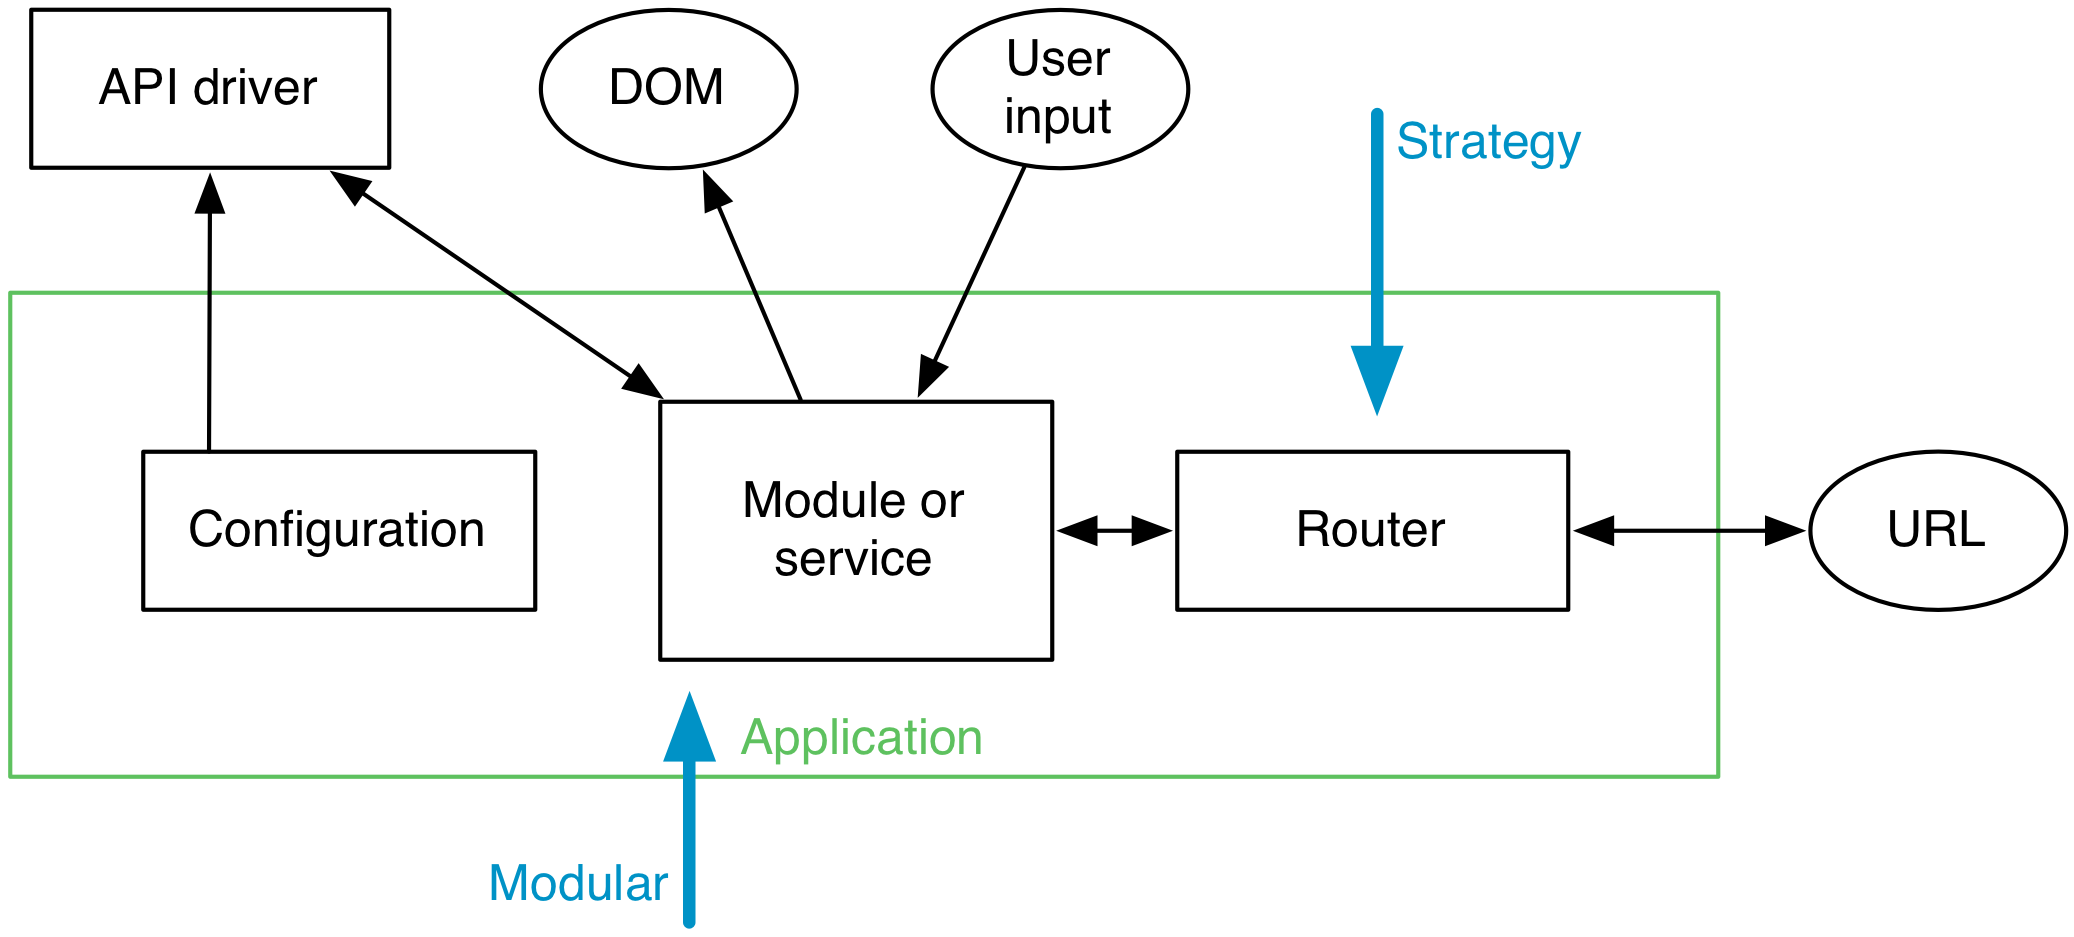
\includegraphics[width=100mm]{gfx/system_design_app.png}}
	\caption{The architecture seen from an application-level.}
	\label{fig:arch_app}
\end{figure}

The idea is that the application will only run one module at a time. When a module is loaded the already active module is unloaded and its memory is released. This makes the application more memory-efficient as well as requiring the developer to think in terms of modules. Modules are supposed to deal with functionality that are page-specific for the site since each module typically implements a group of related features in the application. To deal with components that are used across the entire system services are introduced. A service is just like a module, except for one important difference. An application can run several services at a time where each service can be utilized by modules to perform common tasks in the system. Since the system only needs to run one single instance of each service the singleton pattern is used. This will ensure that the same instance is used across the whole system.

At this level the system can basically be seen as a number of modules that can be loaded and unloaded depending on the URL. It would now be possible to write a module for one project and then move it to another one later on. As long as the module can function by itself it will work there without any changes at all. This is why it is so important that a module can function by itself, all communication is done via a well defined interface which is the same independently on which application is running the module. However, a module can itself be quite complex, so a good module structure is still needed. The design must be further refined.

\subsection{Module-level architecture}

To refine the module structure even further its interface can be analyzed. A module will typically be required to handle data from the API, render HTML-views as well as take care of the user's input. Since the architecture targets smaller applications two-way data bindings would be overkill to use, if the framework would handle all needed bindings it would simply affect the performance too much. With this in mind the MVVM pattern is not really an alternative to use since it is especially designed for using two-way data bindings. A compound of patterns based on MVC would on the other hand work well. MVC was designed to get low coupling between components which of course is an important property to consider a modular system.

However, properties associated with a specific view are an issue with the traditional MVC pattern. In a Javascript implementation the view would represent an HTML-template, which definitely shouldn't be responsible for storing properties related to the presentation since this simply would mix logic and presentation too much. One alternative is to let the controller hold these properties. However, by doing so would make it responsible for several views and would tightly couple them together. Another solution to the problem is to introduce a presentation model in between the controller and the view. The presentation model handles all the UI-properties while the view can focus on rendering UI-elements. By letting the presentation model wrap all the model-objects into property-objects UI-specific properties can be added. This gives a better abstraction even though there now is another component to take into account. When using a presentation model the view now can be implemented with a template language, like Underscore.js or Handlebars.js, while the presentation model can be represented by a component that handles the state of the view. This would remove the dependency between the controller and the views and at the same time allow for a flexible way of dealing with UI-properties.

In traditional MVC the controller would be responsible for taking decisions based on the user input. However, letting the controller be responsible for listening on user input would become problematic in a web-based architecture. User actions are triggered on a DOM-element in the view. This would tightly couple the controller with the view and simply by-pass the presentation model. By instead going towards an MVP concept and let the presentation model handle the user input would keep the abstraction intact. Via a message channel the presentation model can report upwards to the controller that a certain action has occurred. By doing so a decision can be taken by the controller which is implementing the strategy pattern.

Another advantage of introducing the presentation model is that the testability is improved. This is the case since a unit test now can send a message to the controller via the message channel that a user has clicked a button. The unit test can then verify that the right actions are performed by looking at the data structure and see that it has changed. Most of the features of the application can therefore be tested during development with simple unit tests without interacting with the user interface at all.

By wrapping several models into collections and implementing the composite pattern operations can be performed on several models at a time. This can be quite useful since lists of data objects tend to be common in web applications. A presentation model can observe an entire collection of models to get informed whenever there is a change in a model. By utilizing collections operations such as sorting, filtering and pagination are also easy to implement and use.

In order to handle more complex views that might need to be divided into subviews is the composite pattern implemented. By using this pattern a view can be structured like a tree where each node can have other subviews as leafs. Since the DOM itself is represented by a tree-structure containing nodes of DOM-elements it is a highly feasible pattern to use for this purpose.

% TBD: \hl{Write something about module communication. Also mention that presentation models and views comes in pair?}

An illustration of the structure of a module can be seen in figure \ref{fig:arch_module}.

\begin{figure}[h!]
	\centerline{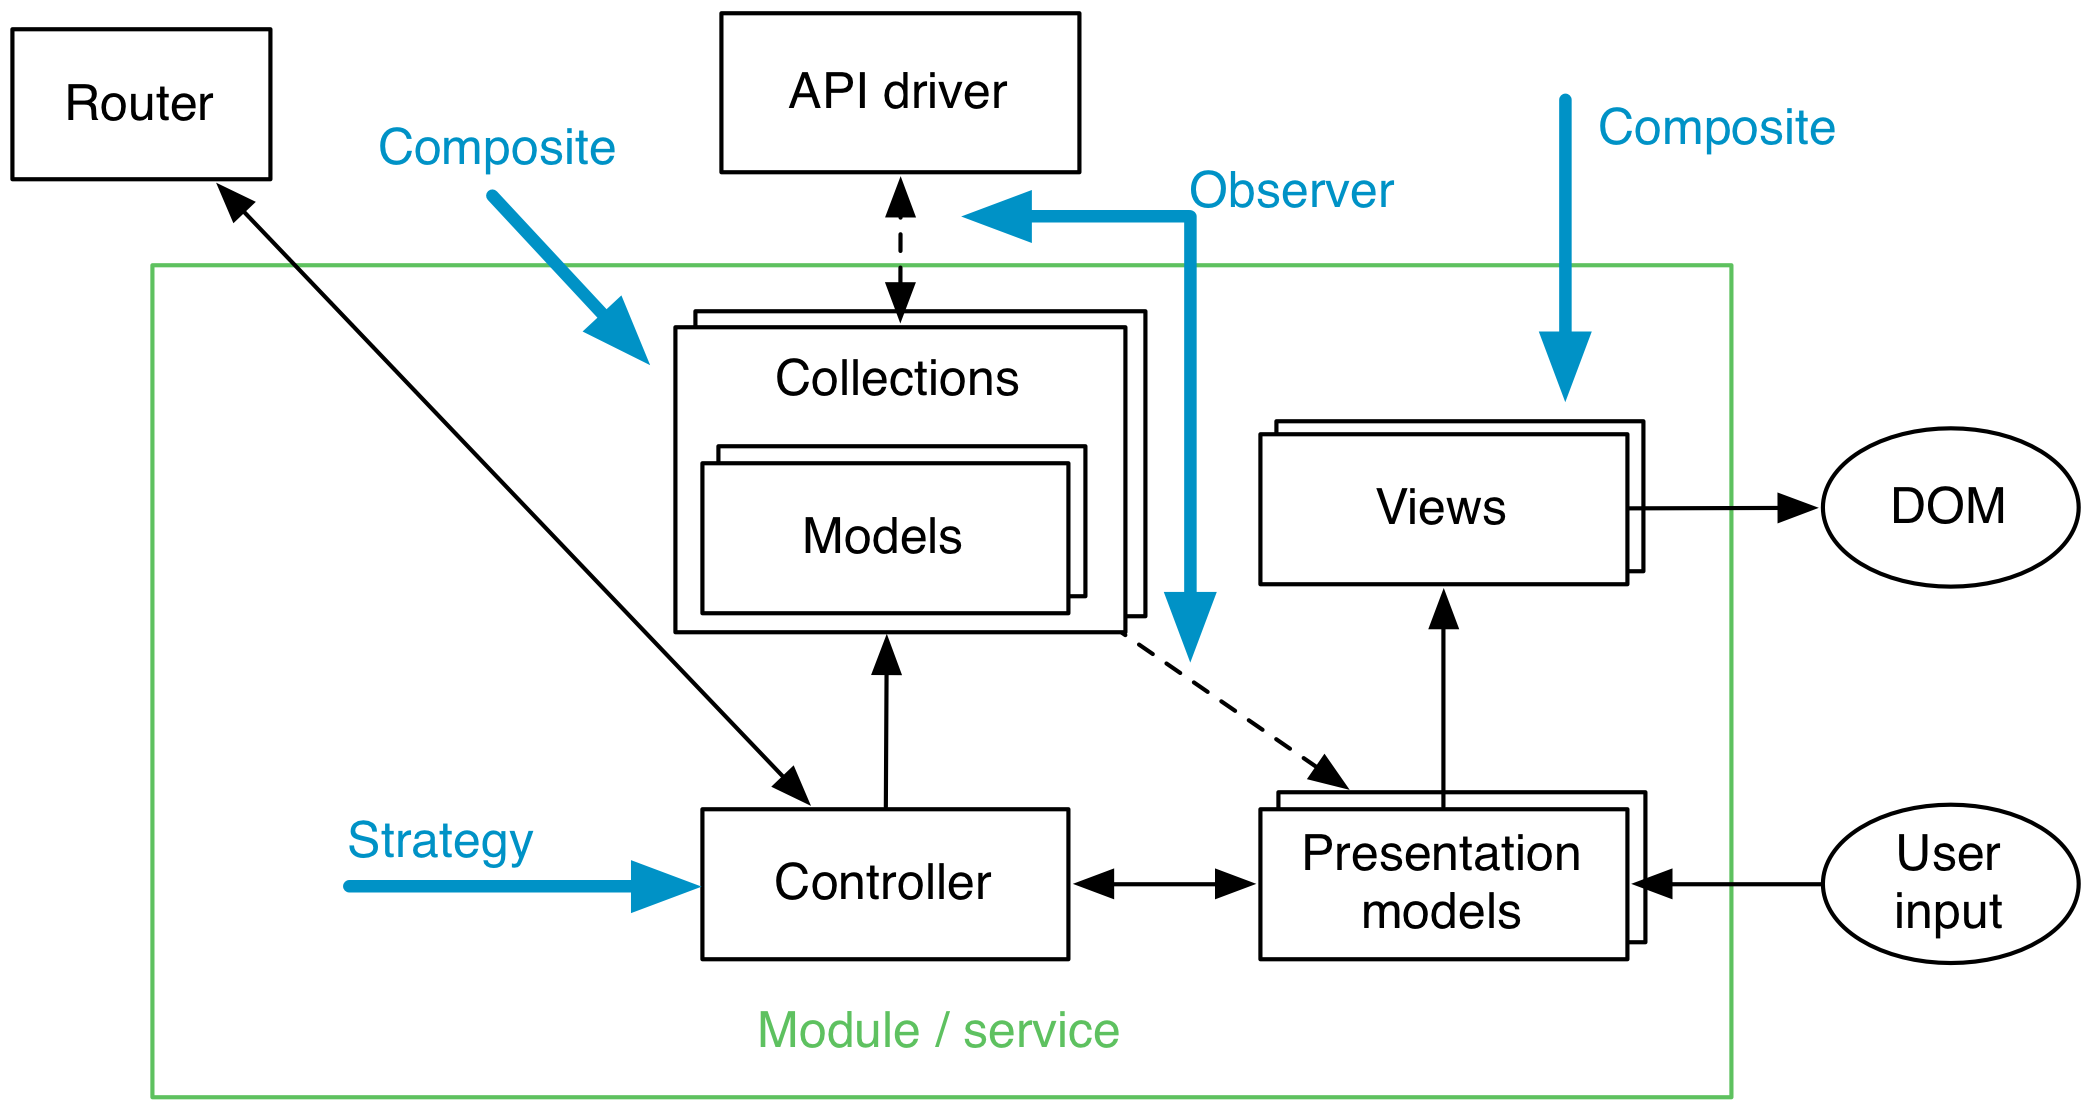
\includegraphics[width=100mm]{gfx/system_design_module.png}}
	\caption{An abstract view of a module/service in the application.}
	\label{fig:arch_module}
\end{figure}

\subsection{API communication}

In order to make the frontend independent on what backend is being used an API driver is introduced. The API driver works as a bridge between the Javascript application and the backend API. It is responsible for implementing a number of methods such as fetch, insert, update and remove. The API driver can be shared between projects since it is typically based on a number of API properties, as long as these properties are the same for two projects the driver will be compatible with both of them. Examples of properties are data transportation (REST, SOAP etc.), data format (JSON, XML etc.) and how the data is to be transferred (AJAX, websockets etc.). The main advantage with an API driver is that if one of these properties are changed a patch is only needed in the API driver, the entire application is not directly affected. For many other frameworks that are lacking support for API drivers it would typically be required to re-write major parts of the application to support the new set of API properties. Another advantage is that frontend developers can start developing the application before the final version of the API is finished. They can for example use an API driver for local storage during the initial development phase and then switch to a driver that is adapted for the API as soon as it is finished. This would allow the frontend to be developed in parallel with the backend. The drawback with having an API driver is some performance loss since it introduces another layer in the architecture. However, this delay can in most cases be neglected since it is really small compared to the time it takes to transfer the message to the server.

\subsection{Initial loading time}

As briefly mentioned in the introduction the initial loading time is a crucial metric to consider. The initial loading time is measured from the time the user has entered the URL in the browser until the page is rendered. Studies shows that 25\% of the users close a page if it takes more than 4 seconds to load, and typically slow pages are less popular \cite{slow_not_pop}. In order to minimize the initial loading time the process can be divided into a number of phases. For SPAs the phases are as follows:

\begin{enumerate}
	\item A user enters the URL in the browser
	\item The page is downloaded
	\item The Javascript is downloaded
	\item The Javascript is parsed
	\item The application is initialized
	\item A module is loaded
	\item If data from the database is needed, it is fetched
	\item The page is rendered
\end{enumerate}

The flow for SPAs can be compared to the flow for traditional sites that only got phase 1, 2, and 8. Hence traditional websites will perform better. It is essential that each and every phase in this flow is executed as fast as possible to minimize the total loading time. The developers can take action as soon as the application is loaded and for example present a loading screen. Once the data is fetched the loading screen can be replaced with the real page that the user requested. To keep the file size down it is essential to minimize the time it takes to download and parse the Javascript. Features that are not used by all applications should not be bundled together with the framework, it would simply make the framework bigger than needed. By using a flexible dependency-handling the framework can be configured so that no unnecessary libraries are included.

\subsection{Search engine optimization}

To approach the problems with crawlers having difficulties running Javascript there are three methods that are widely used:

\begin{itemize}
	\item Crawler-specific HTML snapshots
	\item Share templates between front- and backend
	\item Don't care about crawlers and make no further search engine optimizations
\end{itemize}

Unfortunately have all of these methods a few drawbacks. If crawler-specific HTML snapshots are generated, then there are two versions of the system to maintain. For every change on the site an implementation is required in both the normal Javscript-based system as well as in the system used by the crawler. This generates a lot of duplication of work, which obviously leads to higher maintenance costs.

The other solution, that is slightly more sophisticated, is to re-use the frontend templates on the backend side. Some template languages, such as Mustache, can be rendered in a wide range of languages. Javascript can be used to render the templates on the frontend, while other languages such as Ruby, Python or PHP can be used to render the templates on the backend \cite{mustache}. However, even with this solution there exists duplication of work. The router that maps a URL to a given view must now be maintained on both frontend and backend. The API used by the frontend might not be suitable to use directly by the backend, which in that case would requires a bridge layer in between. This layer must now be maintained for every change in the API that is carried through. It also restricts the choice of template language to an alternative that supports both backend and frontend rendering, which is not a very common property of a template language. One could of course argue that if the backend is written in Javascript, like in Node.js, then the same template language can be used both at the front- and backend. Since there are several alternatives for this setup, it would allow a more flexible choice of template language. However, it now restricts the backend to be written in Javascript which certainly is not a suitable choice in all situations.

Not to care about crawlers at all might sound like a bad idea, but it is important to point out not that all websites need to care about search engines. Examples are internal intranets or systems that require authentication, who do not care about whether public users find them or not. That is simply not their purpose.

\subsubsection{A new approach}
\label{sec:seo_a_new_approach}

A more flexible solution is to write an API that for a given URL downloads the site, executes the Javascript, and then returns the output. When the crawler visits the site a call is made to the API, which generates a snapshot of the site that can be presented to the crawler. The crawler will not be able to distinguish this from the more traditional solution when HTML-snapshots are generated directly by the backend. The flow of communication is illustrated in figure \ref{fig:flow_phantom} and a more detailed description follows below:

\begin{enumerate}
\item The crawler wants to index http://site.com/\#!/subpage
\item The crawler recognizes that the URL contains a hashbang and translates it to http://site.com/?\_escaped\_fragment\_=subpage
\item The webserver sees that the visitor is a crawler since the GET parameter \\$\_escaped\_fragment\_$ is set
\item A request to the Javascript-render API is made with the URL  http://site.com/\#!/subpage as parameter
\item The Javascript-render API visits the given URL and waits for the Javascript to be executed.
\item The Javascript render-API returns a snapshot of the output that is generated
\item The webserver takes the output from the Javscript-render API and provides this to the crawler
\end{enumerate}

\begin{figure}[h!]
	\centerline{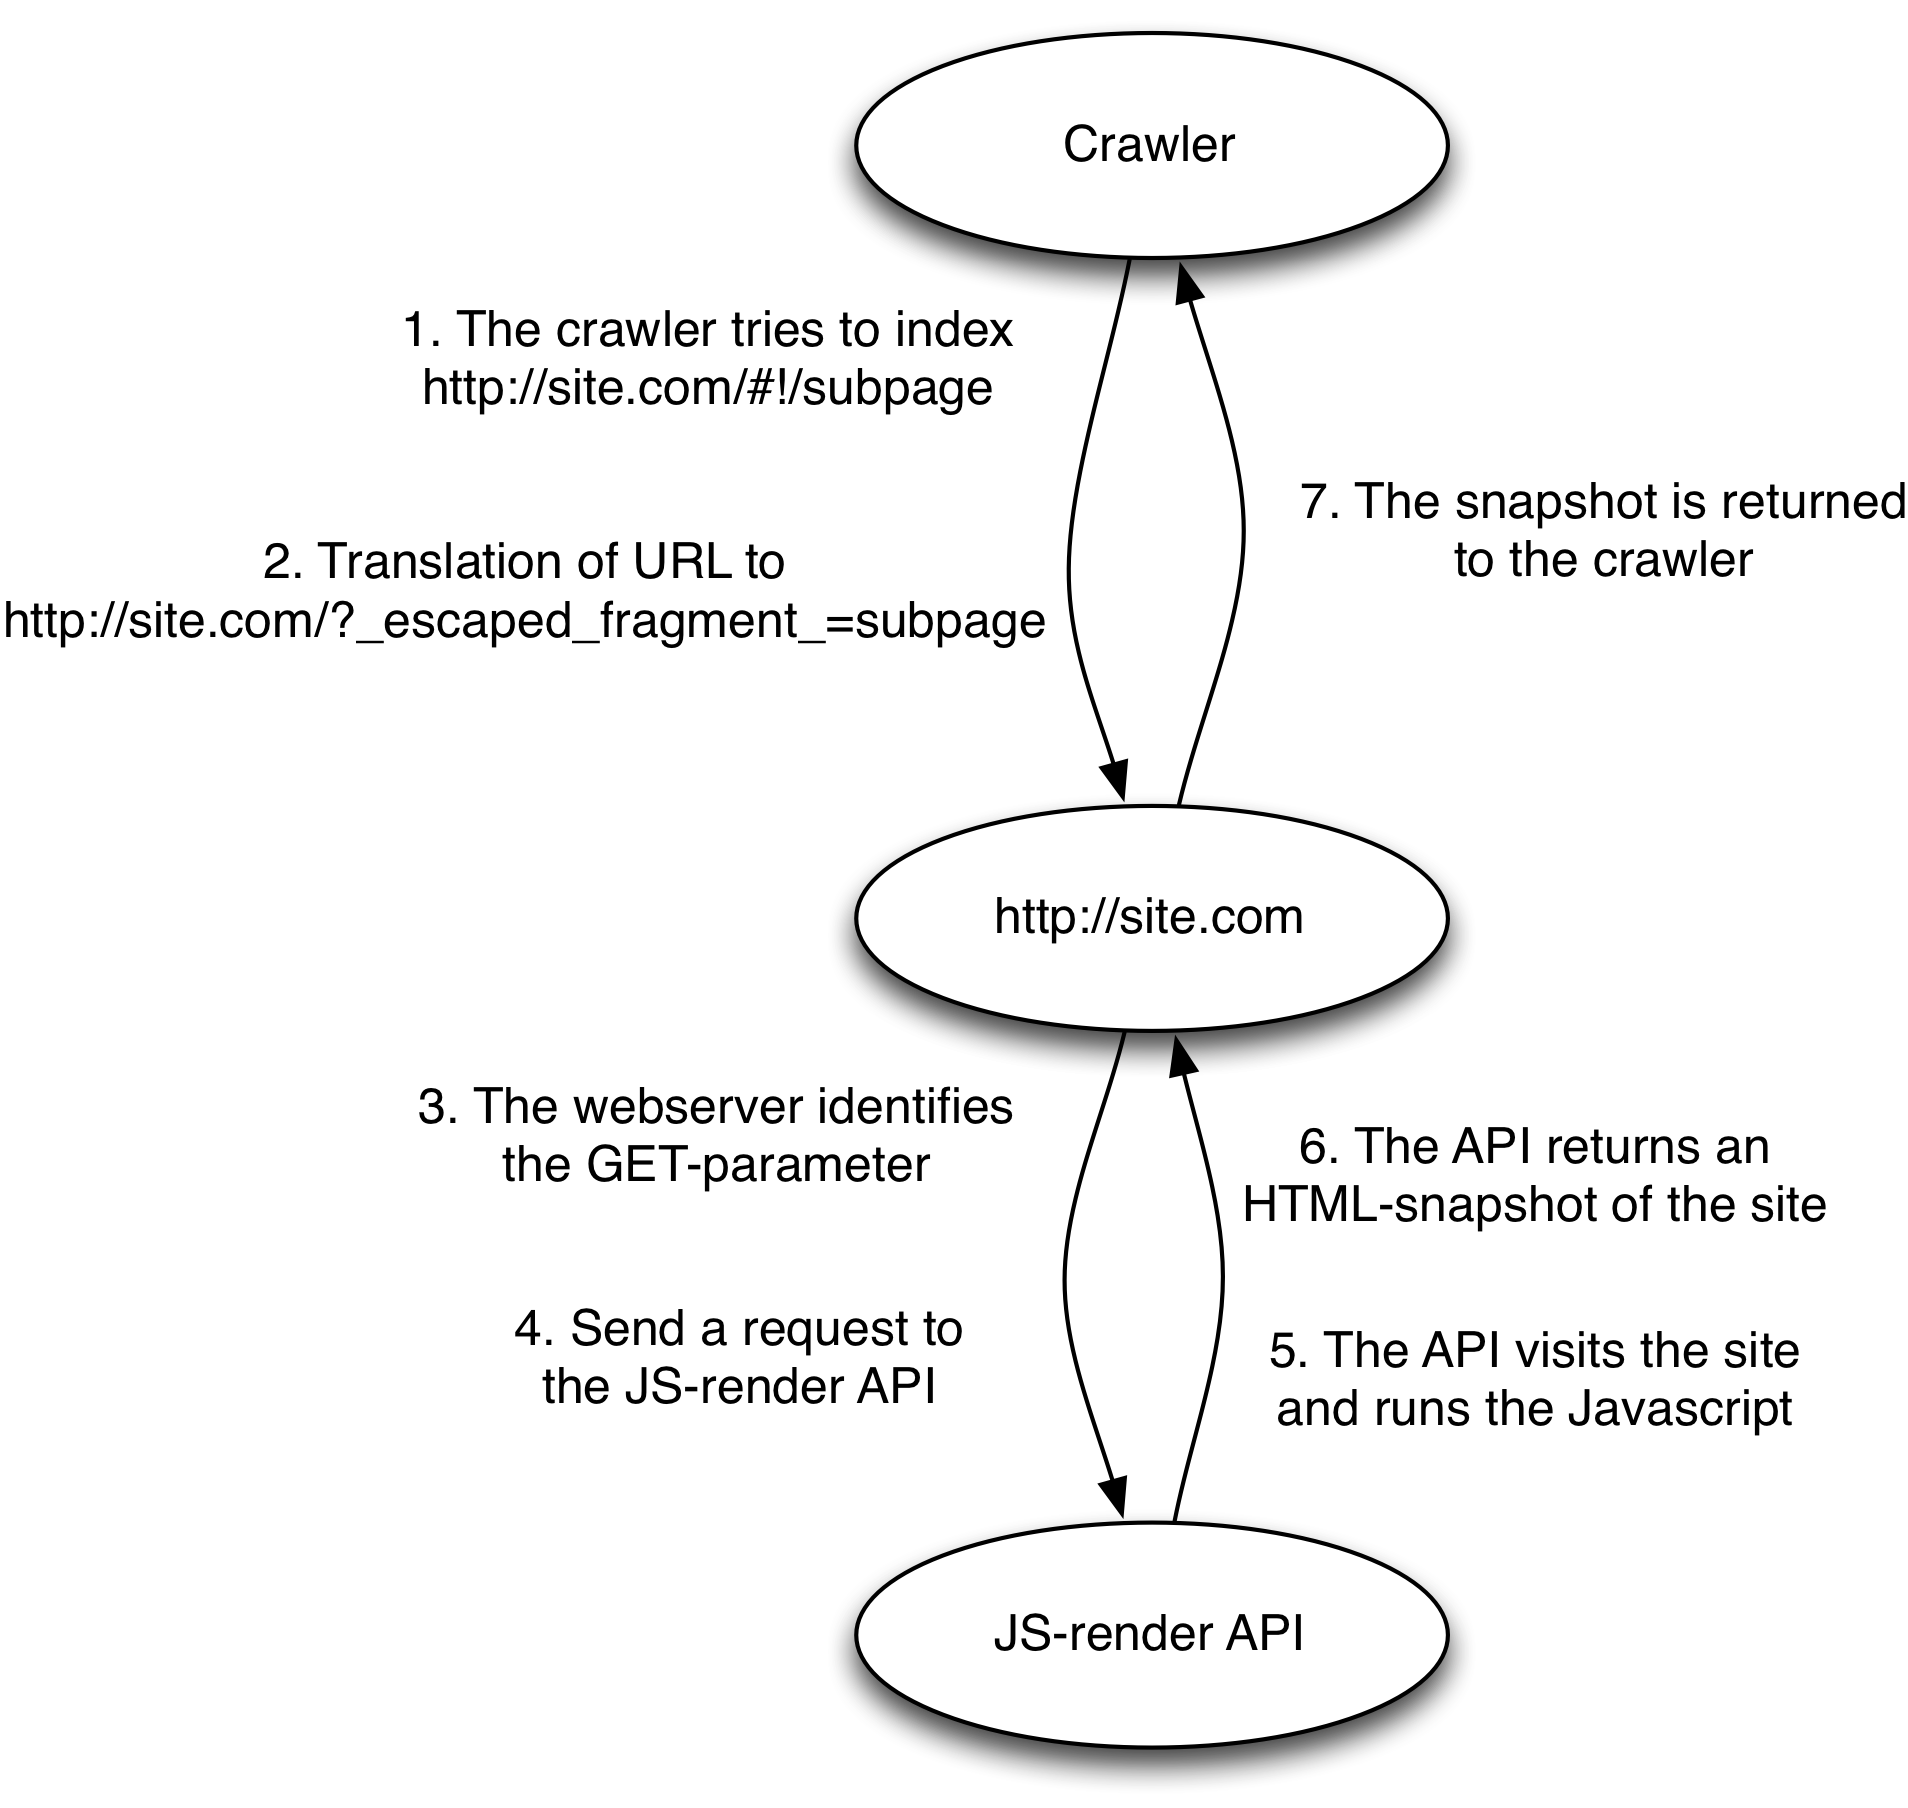
\includegraphics[width=90mm]{gfx/seo_flow_phantom.png}}
	\caption{The flow of communication when using an API for HTML snapshot generation.}
	\label{fig:flow_phantom}
\end{figure}

 This would only require one version of the system to be maintained, that is the normal Javascript-based site. No duplication of work for each view is neither needed, one single solution can be used for the entire site. There are however a number of drawbacks with this solution:

 \begin{itemize}
	\item It heavily depends on the render API. If it crashes it will directly affect the output to the crawler.
	\item The response time for the crawler's request is delayed. There are now more tasks that have to be completed before the crawler gets the output. Especially the page rendering is critical since it tends to be quite slow. This may affect the search engines' evaluation since slow pages are in general less popular \cite{slow_not_pop}.
	\item It can be hard for the API to determine when the page is ready since content is often loaded asynchronously. A method to determine when the page is completely loaded is needed.
\end{itemize}

To approach these drawbacks there are a few things that can be done. A cache can be used to store lately generated snapshots in a database. If the cache was recently updated then the page is fetched from there and simply fed to the crawler directly, this would greatly improve the response time. An own crawler can be written and run periodically to continuously refresh the cache. This would ensure that when the real crawler visits the site the cache is up-to-date and a version of the page can be returned instantly. It also makes the system less dependent on the Javascript render-API since if it happens to crash when rendering a page the last version of it can still be used since it is stored in the cache. This assumes of course that the render-API do not crash {\em every} time the page is rendered.

To determine when the page has loaded and all the content is in place options can be sent to the Javascript render-API. For example a DOM-selector can be specified so that whenever the DOM-element matching this selector has got some content the page is considered as ready. For more complex pages this might however not be sufficient, then flags can instead be used. Whenever a flag is set to a given value is the page considered as ready, the Javascript render-API can simply poll the flag until the given value appears. This puts the developer in full control of when the page is ready to be served to the crawler.
